% !TeX program = xelatex
% !TeX encoding = UTF-8
% A living research note. All section texts are in chapters/*.tex.
\documentclass{ctexart}
% !TeX encoding = UTF-8
% Typesetting and mathematical conventions; extend here as needed.
\usepackage[a4paper,left=27mm,right=27mm,top=26mm,bottom=28mm,headheight=15pt]{geometry}
\usepackage{fontspec}
\setmainfont{TeX Gyre Termes}
\setsansfont{TeX Gyre Heros}
\setmonofont{DejaVu Sans Mono}[Scale=0.82]
% ctexart already configures Fandol Chinese fonts (including bold and italic)
% in the cloud XeLaTeX environment; avoid overriding its CJK font families.
\usepackage{amsmath,amssymb,amsthm,mathtools,bm}
\usepackage{graphicx} % Insert figures when experimental figures are added
\usepackage{booktabs,tabularx,longtable,array}
\usepackage{enumitem}
\usepackage{caption}
\usepackage{float}
\usepackage{fancyhdr}
\usepackage{microtype}
\usepackage{xcolor}
\usepackage{listings}
\usepackage{tikz}
\usepackage{pgfplots}
\pgfplotsset{compat=1.18}
\usepackage[backend=biber,style=gb7714-2015,sorting=none,gbnamefmt=lowercase,maxbibnames=7]{biblatex}
\addbibresource{references.bib}
\usepackage[unicode,bookmarksnumbered=true,colorlinks=true,linkcolor=black,citecolor=black,urlcolor=black]{hyperref}

\definecolor{ink}{HTML}{202B36}
\definecolor{accent}{HTML}{344E68}
\definecolor{pale}{HTML}{E8EDF2}
\definecolor{codebg}{HTML}{F5F6F7}
\AtBeginDocument{\color{ink}}
\ctexset{
  section={format=\Large\bfseries\sffamily\color{accent},beforeskip=23pt,afterskip=12pt},
  subsection={format=\large\bfseries\sffamily,beforeskip=15pt,afterskip=7pt},
  subsubsection={format=\normalsize\bfseries\sffamily,beforeskip=11pt,afterskip=5pt}
}
\setlength{\parindent}{2em}
\setlength{\parskip}{2pt}
\linespread{1.25}
\setlist[itemize]{leftmargin=2.2em,itemsep=3pt,topsep=5pt}
\setlist[enumerate]{leftmargin=2.2em,itemsep=3pt,topsep=5pt}
\captionsetup{font=small,labelfont=bf}
\numberwithin{equation}{section}

\theoremstyle{plain}
\newtheorem{proposition}{命题}[section]
\newtheorem{theorem}[proposition]{定理}
\theoremstyle{definition}
\newtheorem{definition}[proposition]{定义}
\newtheorem{assumption}[proposition]{假设}
\theoremstyle{remark}
\newtheorem{remark}[proposition]{注记}
\renewcommand{\proofname}{证明}

\newcommand{\R}{\mathbb{R}}
\newcommand{\E}{\mathbb{E}}
\newcommand{\Prob}{\mathbb{P}}
\DeclareMathOperator{\Var}{Var}
\DeclareMathOperator{\Bias}{Bias}
\DeclareMathOperator*{\argmin}{arg\,min}
\DeclareMathOperator*{\argmax}{arg\,max}
\newcommand{\norm}[1]{\left\lVert #1\right\rVert}
\newcommand{\abs}[1]{\left\lvert #1\right\rvert}
\newcommand{\trans}{^{\mathsf T}}

\pagestyle{fancy}
\fancyhf{}
\fancyhead[L]{\small\sffamily 机器学习}
\fancyhead[R]{\small\sffamily\nouppercase{\leftmark}}
\fancyfoot[C]{\small\thepage}
\renewcommand{\headrulewidth}{0.35pt}
\fancypagestyle{plain}{\fancyhf{}\fancyfoot[C]{\small\thepage}\renewcommand{\headrulewidth}{0pt}}

\lstdefinestyle{research}{
 language=Python,basicstyle=\ttfamily\footnotesize,backgroundcolor=\color{codebg},
 numbers=left,numberstyle=\tiny\color{gray},numbersep=9pt,
 frame=single,rulecolor=\color{pale},framesep=7pt,
 showstringspaces=false,breaklines=true,tabsize=4,
 keywordstyle=\color{accent}\bfseries,commentstyle=\color{gray},
 xleftmargin=6pt,xrightmargin=4pt,aboveskip=13pt,belowskip=13pt
}
\lstset{style=research}


\title{机器学习}
\author{天国\quad 付}
\date{November 2026}

\begin{document}
\maketitle
\thispagestyle{plain}

\begin{abstract}
本文围绕统计学习中的模型构建、参数估计、数值优化与泛化评估，整理基础定义、主要公式及其推导条件。讨论以线性回归和二分类概率模型为主，同时记录梯度下降的数学性质、模型评估的常用方法与可复现的数值算例。文稿按照研究问题组织，而非课堂顺序；后续将逐步补充正则化、优化算法及相关实验。
\end{abstract}
\noindent\textbf{关键词：}统计学习；最小二乘；梯度下降；逻辑回归；泛化误差

\tableofcontents
\clearpage

\section{引言}\label{sec:introduction}

这份笔记只整理机器学习入门阶段最常用的概念、公式与方法。重点是三个问题：\textbf{模型怎样预测、参数怎样求、效果怎样评价}。

正文依次介绍基本概念、线性回归、梯度下降、逻辑回归和模型评价。每节保留核心公式及必要条件，省略重复推导和暂时用不到的定理。数值例子与 Python 脚本用于辅助理解。

主要参考周志华《机器学习》、李航《统计学习方法》和 \textit{An Introduction to Statistical Learning}\cite{zhou2016,lihang2019,james2023}。
\section{从数据到优化问题}\label{ch:foundations}

\subsection{统计学习的对象}

考虑训练数据
\begin{equation}\label{eq:dataset}
D=\{(x_i,y_i)\}_{i=1}^{m},\qquad x_i\in\mathcal X,\quad y_i\in\mathcal Y.
\end{equation}
其中 $x_i$ 为输入、$y_i$ 为目标变量，$m$ 为样本数。若输入是 $p$ 维数值向量，则 $x_i\in\R^p$。监督学习利用输入与目标之间的对应关系估计预测函数；无监督学习通常只有输入数据，其目标是发现数据的结构，例如聚类或低维表示\cite[第1章]{zhou2016}。

对监督学习而言，回归任务的目标变量通常是连续数值；分类任务的目标变量是有限个类别。分类器可以输出类别，也可以先输出类别的条件概率，再根据决策规则得到最终类别。\emph{是否使用梯度下降并不决定任务类型}；任务类型取决于待预测的变量和问题设定。

以简单线性模型为例，假设类为
\begin{equation}\label{eq:linear-family}
\mathcal F=\{f_{w,b}(x)=wx+b:\;w,b\in\R\}.
\end{equation}
模型族 $\mathcal F$ 规定允许采用怎样的函数形式；参数 $w,b$ 选择其中一个具体模型；优化算法则确定怎样利用数据求得参数。三者在概念上应当分开。

\subsection{损失函数和经验风险}

预测结果未必与观测值相同，需要用损失函数 $L(y,\hat y)$ 量化差异。常见的回归损失为平方损失
\begin{equation}\label{eq:squared-loss}
L(y,\hat y)=(y-\hat y)^2.
\end{equation}
在有限样本上取平均，得到经验风险
\begin{equation}\label{eq:empirical-risk}
\widehat R_D(f)=\frac1m\sum_{i=1}^{m}L\bigl(y_i,f(x_i)\bigr).
\end{equation}
因此，经验风险最小化（empirical risk minimization, ERM）可以写成
\begin{equation}\label{eq:erm}
\hat f\in\argmin_{f\in\mathcal F}\widehat R_D(f).
\end{equation}
式 \eqref{eq:erm} 说明学习问题如何转化为优化问题，但没有规定一定使用哪种算法。对可以直接求解的模型，可使用解析方法；对难以得到闭式解的模型，常考虑数值迭代方法。

平方损失的优点在于非负、连续可微，且有利于构造最小二乘问题；不足之处是较大的残差会受到二次惩罚，因此估计结果可能对异常值较敏感。损失函数并非只有一种，后文讨论二分类时将使用由概率模型导出的对数损失。

\subsection{经验风险与总体风险}

若数据来自未知联合分布 $P_{X,Y}$，则可定义总体风险
\begin{equation}\label{eq:population-risk}
R(f)=\E_{(X,Y)\sim P_{X,Y}}\bigl[L(Y,f(X))\bigr].
\end{equation}
经验风险用样本均值近似总体期望；两者通常并不相等。训练过程直接接触到的是样本，而预测最终面向未知观测，这种差别是泛化问题的起点\cite[第1章]{lihang2019}。

\begin{proposition}[固定预测函数时经验风险的无偏性]\label{prop:fixed-risk}
设 $Z_i=(X_i,Y_i)$ 独立同分布，且 $\E\abs{L(Y,f(X))}<\infty$。若预测函数 $f$ 在观测该训练样本之前已固定，则
\begin{equation}
\E_D\bigl[\widehat R_D(f)\bigr]=R(f).
\end{equation}
\end{proposition}
\begin{proof}
由期望的线性性及相同分布，
\[
\E_D\left[\frac1m\sum_{i=1}^mL(Y_i,f(X_i))\right]
=\frac1m\sum_{i=1}^m\E[L(Y_i,f(X_i))]=R(f).
\]
此处不需要各损失项彼此独立才能使用期望线性性；独立同分布是给定的典型抽样假设。
\end{proof}

\begin{remark}
命题 \ref{prop:fixed-risk} 的关键是 $f$ 在样本被观察前已固定。训练所得的 $\hat f_D$ 依赖于同一批数据，不能把它不加区别地代入上述证明；否则容易错误地认为训练误差天然就是泛化误差的无偏估计。
\end{remark}

\subsection{一个不依赖数值优化器的例子}

对于 $D=\{(1,2),(2,4),(3,6)\}$，考虑过原点的线性模型 $f_w(x)=wx$。其均方误差为
\begin{align}
\widehat R_D(w)
&=\frac13\bigl[(w-2)^2+(2w-4)^2+(3w-6)^2\bigr]\\
&=\frac{14}{3}(w-2)^2.
\end{align}
由完全平方的非负性可知 $\widehat R_D(w)\ge 0$，且等号仅在 $w=2$ 时成立。因此 $w^*=2$ 是唯一全局最小点，最优值为零。这个例子说明：建立优化问题和选择求解算法是两件事。这里直接观察平方项即可求解，无须调用梯度下降。

\subsection{保留的问题}

经验风险最小化何时能得到接近总体风险最小值的模型？这一问题依赖函数类的复杂度、抽样假设及评价方法，不能仅凭目标函数的最优值回答。相关讨论放在第\ref{ch:generalization}节，并在今后的学习中继续补充更严格的泛化界。

\section{线性回归与最小二乘法}\label{ch:least-squares}

\subsection{核心思路}

对于一元线性回归，预测式为 $\hat y_i=wx_i+b$。最小二乘法选择让误差平方和最小的 $w,b$：
\begin{equation}\label{eq:linear-objective}
\boxed{J(w,b)=\frac1{2m}\sum_{i=1}^{m}(wx_i+b-y_i)^2.}
\end{equation}
系数 $1/2$ 方便求导，不影响最优参数；实际报告的 MSE 则不包含这个 $1/2$。

\subsection{怎样直接求出直线}

记 $\bar x$ 为所有 $x_i$ 的平均值，$\bar y$ 为所有 $y_i$ 的平均值。对 $w,b$ 求偏导并令其为零，得到
\begin{equation}\label{eq:slope-ls}
\boxed{\hat w=
\frac{\sum_{i=1}^{m}(x_i-\bar x)(y_i-\bar y)}
     {\sum_{i=1}^{m}(x_i-\bar x)^2},
\qquad
\hat b=\bar y-\hat w\bar x.}
\end{equation}

\textbf{使用条件：}至少有两个不同的 $x_i$，否则分母为零，无法唯一确定斜率。这个公式说明拟合直线一定经过 $(\bar x,\bar y)$\cite[第3章]{james2023}。

\subsection{一个小例子}

给定 $(1,2),(2,3),(3,5)$，有 $\bar x=2,\ \bar y=10/3$。代入公式得到
\[
\hat w=\frac32,\qquad \hat b=\frac13,
\]
所以拟合直线是 $\hat y=\frac32x+\frac13$。对应的 MSE 为 $1/18$。

\subsection{需要注意什么}

最小二乘法求的是\textbf{训练数据上的最佳拟合直线}，不保证因果关系，也不保证对新数据预测得好。它不要求误差一定服从正态分布；正态假设主要用于进一步进行统计推断或似然解释。

多个特征也可以做线性回归，但会用到矩阵计算。入门阶段先掌握上述一元公式即可。
\section{一阶优化方法：梯度下降与步长}\label{ch:gradient}

\subsection{迭代法的出发点}

最小二乘问题在适当的秩条件下可以写出显式解，但许多优化目标没有便于直接计算的闭式解。对可微函数 $J:\R^p\to\R$，考虑
\[
\min_{\theta\in\R^p}J(\theta).
\]
迭代方法从初值 $\theta_0$ 出发，构造 $\theta_1,\theta_2,\ldots$，希望目标函数逐步下降，最终得到近似最优解。需要区分两个概念：\emph{下降方向}决定局部朝哪里移动，\emph{步长}决定一次移动多远。即便方向正确，过大的步长仍可能使函数值上升。

\subsection{方向导数与负梯度}

若 $J$ 在 $\theta$ 处可微，沿单位方向 $d$ 的方向导数为
\begin{equation}\label{eq:directional-deriv}
D_dJ(\theta)=\nabla J(\theta)\trans d,\qquad \norm d_2=1.
\end{equation}
依据 Cauchy--Schwarz 不等式，
\[
\nabla J(\theta)\trans d\ge-\norm{\nabla J(\theta)}_2.
\]
当 $\nabla J(\theta)\ne0$ 时，取
\begin{equation}\label{eq:steepest-descent-direction}
d_*=-\frac{\nabla J(\theta)}{\norm{\nabla J(\theta)}_2}
\end{equation}
达到上述下界。因此负梯度是\emph{欧氏范数下局部一阶变化率最小的单位方向}。这里的“最速”是局部概念，不意味着一步更新就达到全局最优点，也不保证任意步长均能下降\cite[第5章]{liu2020}。

梯度下降法把方向与步长结合起来，得到
\begin{equation}\label{eq:gd-update}
\boxed{\theta_{k+1}=\theta_k-\eta_k\nabla J(\theta_k),\qquad \eta_k>0.}
\end{equation}
对于含斜率和截距的模型，应先在 $(w_k,b_k)$ 处计算梯度，再同步更新这两个参数。

如果在一次迭代中先更新 $w$，再用新的 $w$ 更新 $b$，得到的便是另一种顺序更新方法。

\subsection{线性回归中的梯度}

对含截距的简单线性回归，
\[
J(w,b)=\frac1{2m}\sum_{i=1}^{m}(wx_i+b-y_i)^2.
\]
由链式法则，
\begin{equation}\label{eq:gd-lm-partials}
\frac{\partial J}{\partial w}=\frac1m\sum_{i=1}^{m}(wx_i+b-y_i)x_i,\quad
\frac{\partial J}{\partial b}=\frac1m\sum_{i=1}^{m}(wx_i+b-y_i).
\end{equation}
对应的同步更新为
\begin{align}
w_{k+1}&=w_k-\frac{\eta_k}{m}\sum_i(w_kx_i+b_k-y_i)x_i,\\
b_{k+1}&=b_k-\frac{\eta_k}{m}\sum_i(w_kx_i+b_k-y_i).
\end{align}

取 $D=\{(1,2),(2,4)\}$，以 $(w_0,b_0)=(0,0)$ 为初值，可算得 $\partial_wJ=-5$、$\partial_bJ=-3$。取 $\eta_0=0.1$，一步后参数为
\begin{equation}\label{eq:gd-first-step}
(w_1,b_1)=(0.5,0.3).
\end{equation}
这只是一次迭代的结果，而非最优解。将其代入损失函数，可以检查此次更新是否确实实现了下降。

\subsection{学习率与一个可完整分析的例子}

考虑一元二次目标
\begin{equation}\label{eq:scalar-quadratic}
J(w)=(w-2)^2.
\end{equation}
其唯一最小点为 $w_*=2$。因 $J'(w)=2(w-2)$，梯度下降满足
\[
w_{k+1}-2=(1-2\eta)(w_k-2).
\]
若学习率 $\eta$ 固定，则递推得到
\begin{equation}\label{eq:gd-error-recursion}
w_k-2=(1-2\eta)^k(w_0-2).
\end{equation}
对任意初值的收敛充要条件为 $\abs{1-2\eta}<1$，也就是
\begin{equation}\label{eq:scalar-gd-range}
\boxed{0<\eta<1.}
\end{equation}
$\eta=1/2$ 时，除初值已为最优点外，迭代一步即可到达 $w_*$；$\eta=1$ 时通常发生两点振荡；$\eta>1$ 时，除最优初值外，误差绝对值增大。这些判断只对当前目标成立，不能直接拿来作为一般优化问题的步长条件。

\begin{figure}[htbp]
\centering
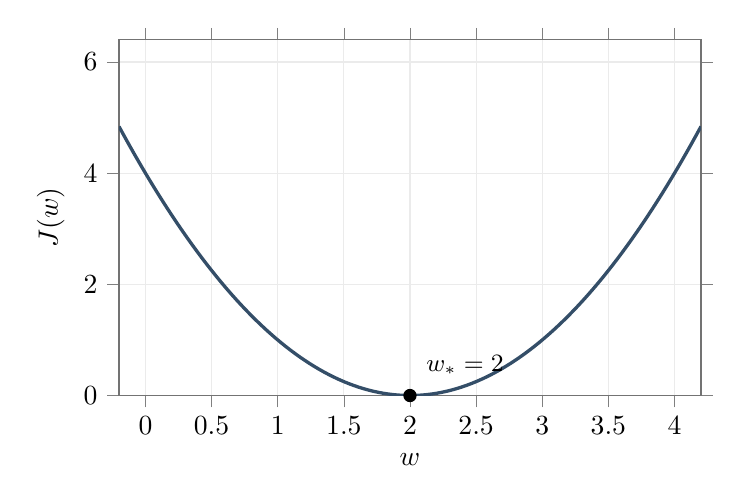
\begin{tikzpicture}
\begin{axis}[width=.74\textwidth,height=6.1cm,xlabel={$w$},ylabel={$J(w)$},xmin=-.2,xmax=4.2,ymin=0,ymax=6.4,grid=major,grid style={draw=gray!16},axis line style={draw=black!55},tick align=outside]
\addplot[very thick,color=accent,domain=-.2:4.2,samples=120]{(x-2)^2};
\addplot[only marks,mark=*,mark size=2.2pt,color=black] coordinates {(2,0)};
\node[anchor=south west,font=\small] at (axis cs:2.05,.2) {$w_*=2$};
\end{axis}
\end{tikzpicture}
\caption{二次目标 $J(w)=(w-2)^2$。曲线的极小点可以解析确定；梯度下降能否接近该点取决于步长。}\label{fig:quadratic-objective}
\end{figure}

\subsection{一般光滑目标的下降估计}

为了从简单例子走向一般结论，加入一个常见条件。

\begin{assumption}[$L$-光滑]\label{ass:smooth}
函数 $J$ 连续可微，且存在常数 $L>0$，使任意 $u,v\in\R^p$ 满足
\begin{equation}
\norm{\nabla J(u)-\nabla J(v)}_2\le L\norm{u-v}_2.
\end{equation}
\end{assumption}

\begin{proposition}[下降引理]\label{prop:descent-lemma}
在假设 \ref{ass:smooth} 下，任意 $u,v$ 满足
\begin{equation}\label{eq:descent-lemma}
J(v)\le J(u)+\nabla J(u)\trans(v-u)+\frac L2\norm{v-u}_2^2.
\end{equation}
\end{proposition}
\begin{proof}
令 $d=v-u$，定义 $g(t)=J(u+td)$。由微积分基本定理，
\[
J(v)-J(u)=\int_0^1\nabla J(u+td)\trans d\,\mathrm dt.
\]
减去 $\nabla J(u)\trans d$，并利用 Cauchy--Schwarz 不等式及梯度的 Lipschitz 条件，
\begin{align*}
&J(v)-J(u)-\nabla J(u)\trans d\\
&=\int_0^1[\nabla J(u+td)-\nabla J(u)]\trans d\,\mathrm dt\\
&\le\int_0^1 Lt\norm d_2^2\,\mathrm dt
=\frac L2\norm d_2^2.
\end{align*}
即得结论。
\end{proof}

在式 \eqref{eq:descent-lemma} 中令 $v=u-\eta\nabla J(u)$，得到
\begin{equation}\label{eq:gd-descent-estimate}
J(u-\eta\nabla J(u))\le J(u)-\eta\left(1-\frac{L\eta}{2}\right)\norm{\nabla J(u)}_2^2.
\end{equation}
因而当 $0<\eta<2/L$ 时，若梯度非零，右侧严格小于 $J(u)$。特别是 $\eta\le1/L$ 时有便于使用的下降下界。\textbf{函数值下降并不单独保证迭代点收敛到全局最优点}；要得出更强结论，还需要目标函数的下界、凸性或其他条件。

\subsection{凸性、驻点与全局最优}

若 $J$ 是可微凸函数，则其一阶条件为
\[
J(v)\ge J(u)+\nabla J(u)\trans(v-u).
\]
因此 $\nabla J(u_*)=0$ 蕴含 $J(v)\ge J(u_*)$ 对任意 $v$ 成立，即 $u_*$ 是全局最小点。反之，对于定义在整个 $\R^p$ 上的可微函数，任意局部极小点均满足梯度为零。两者合起来说明：\emph{对于无约束可微凸优化，驻点与全局最小点等价。}

非凸情形不能照搬这一结论。例如 $J(w)=-w^2$ 在 $w=0$ 处梯度为零，但该点是局部最大点。实际算法分析必须说明所用结论属于哪一类目标函数。

\subsection{后续扩展}

当前主要使用固定步长讨论梯度下降。今后可以补充精确线搜索、回溯线搜索、强凸函数的线性收敛，以及牛顿法、拟牛顿法与随机梯度方法，并比较每步代价和精度要求。

\section{二分类的概率建模与对数损失}\label{ch:logistic}

\subsection{从线性得分到条件概率}

考虑二分类标签 $Y\in\{0,1\}$，线性得分 $z=x\trans\beta$ 可取任意实数，因此不能直接作为概率。逻辑回归使用 Logistic 函数
\begin{equation}\label{eq:sigmoid}
\sigma(z)=\frac{1}{1+\mathrm e^{-z}}
\end{equation}
把实数映射到开区间 $(0,1)$，并定义
\begin{equation}\label{eq:logistic-model}
\pi(x)=\Prob(Y=1\mid X=x)=\sigma(x\trans\beta).
\end{equation}
其中 $x$ 可以含截距对应的常数分量。这里采用 $\pi$ 表示条件概率，以免与特征维数 $p$ 混淆。

由 \eqref{eq:sigmoid} 可得
\[
\frac{\pi(x)}{1-\pi(x)}=\mathrm e^{x\trans\beta},
\]
因此
\begin{equation}\label{eq:log-odds}
\boxed{\log\frac{\pi(x)}{1-\pi(x)}=x\trans\beta.}
\end{equation}
模型对\emph{对数几率}作线性建模。这也解释了 Logistic Regression 虽然沿用“回归”一词，却主要用于分类任务\cite[第3章]{zhou2016}。

\subsection{Sigmoid 的导数}

对式 \eqref{eq:sigmoid} 求导，
\begin{align}
\sigma'(z)
&=-(1+\mathrm e^{-z})^{-2}(-\mathrm e^{-z})\\
&=\frac{\mathrm e^{-z}}{(1+\mathrm e^{-z})^2}\\
&=\boxed{\sigma(z)[1-\sigma(z)]}.\label{eq:sigmoid-derivative}
\end{align}
因此 Sigmoid 单调递增，且 $0<\sigma'(z)\le1/4$。\textbf{Sigmoid 并不是在整个实数轴上凸的}：其二阶导数符号在 $z=0$ 两侧发生改变。逻辑回归的凸性来自负对数似然关于参数的结构，而非 Sigmoid 函数自身的全局凸性。

\begin{figure}[htbp]
\centering
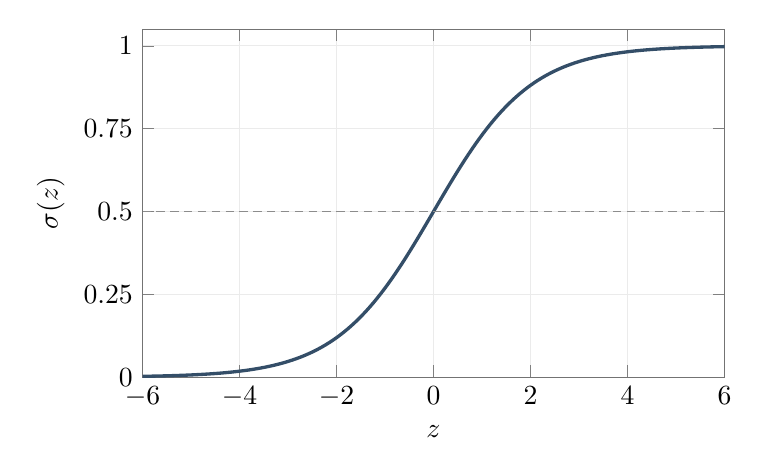
\begin{tikzpicture}
\begin{axis}[width=.74\textwidth,height=6cm,xlabel={$z$},ylabel={$\sigma(z)$},xmin=-6,xmax=6,ymin=0,ymax=1.05,grid=major,grid style={draw=gray!16},ytick={0,0.25,0.5,0.75,1},axis line style={draw=black!55}]
\addplot[very thick,color=accent,domain=-6:6,samples=160]{1/(1+exp(-x))};
\addplot[densely dashed,color=black!45] coordinates {(-6,.5) (6,.5)};
\end{axis}
\end{tikzpicture}
\caption{Logistic 函数将线性得分映射为二分类概率。$z=0$ 时输出为 $0.5$。}\label{fig:sigmoid}
\end{figure}

\subsection{伯努利似然与交叉熵}

对样本 $(x_i,y_i)$，设 $Y_i\mid x_i\sim\operatorname{Bernoulli}(\pi_i)$，其中 $\pi_i=\sigma(x_i\trans\beta)$。在给定输入后，若样本标签条件独立，则条件似然为
\begin{equation}\label{eq:logit-likelihood}
\mathcal L(\beta)=\prod_{i=1}^{m}\pi_i^{y_i}(1-\pi_i)^{1-y_i}.
\end{equation}
取对数、乘以负号并按样本平均，得到
\begin{equation}\label{eq:bce}
\boxed{J(\beta)=-\frac1m\sum_{i=1}^{m}\left[y_i\log\pi_i+(1-y_i)\log(1-\pi_i)\right].}
\end{equation}
这是二元交叉熵，也是该伯努利模型的平均负对数似然。由此可见，在给定概率假设和独立性条件下，损失函数具有明确的统计来源，而不是仅凭曲线形状选择\cite[第6章]{lihang2019}。

\subsection{从链式法则推导梯度}

先考虑一个样本，记
\[
\ell=-y\log\pi-(1-y)\log(1-\pi),\quad\pi=\sigma(z),\quad z=x\trans\beta.
\]
对概率变量求导：
\[
\frac{\partial\ell}{\partial\pi}=-\frac y\pi+\frac{1-y}{1-\pi}
=\frac{\pi-y}{\pi(1-\pi)}.
\]
再利用式 \eqref{eq:sigmoid-derivative}，
\[
\frac{\partial\ell}{\partial z}
=\frac{\partial\ell}{\partial\pi}\frac{\mathrm d\pi}{\mathrm dz}
=\frac{\pi-y}{\pi(1-\pi)}\pi(1-\pi)=\pi-y.
\]
由于 $\nabla_\beta z=x$，因此
\begin{equation}\label{eq:logistic-single-gradient}
\boxed{\nabla_\beta\ell=(\pi-y)x.}
\end{equation}
把所有样本堆叠为设计矩阵 $X\in\R^{m\times p}$，定义概率向量 $\boldsymbol\pi=(\pi_1,\ldots,\pi_m)\trans$，得到平均损失梯度
\begin{equation}\label{eq:logistic-full-gradient}
\boxed{\nabla J(\beta)=\frac1mX\trans(\boldsymbol\pi-y).}
\end{equation}
这里的结构与最小二乘梯度 \eqref{eq:ls-gradient} 十分接近：都是先计算某种“预测与真实值之差”，再乘设计矩阵的转置。差别在于预测值和损失函数来自不同的概率或建模假设。

\subsection{Hessian、凸性与例外情形}

记 $W=\operatorname{diag}\{\pi_i(1-\pi_i)\}_{i=1}^m$，则
\begin{equation}\label{eq:logistic-hessian}
\nabla^2J(\beta)=\frac1mX\trans W X.
\end{equation}
对任意 $v$，
\[
v\trans\nabla^2J(\beta)v=\frac1m(Xv)\trans W(Xv)\ge0,
\]
所以在常规无正则化二分类逻辑回归中，平均负对数似然关于 $\beta$ 是凸函数。对所有有限参数，$\pi_i\in(0,1)$，故 $W$ 的对角元素严格为正；若 $X$ 满列秩，则 Hessian 正定。

但是正定 Hessian 并不自动保证有限的极小点存在。例如样本线性完全可分时，沿某些参数方向把系数绝对值持续放大，可以使负对数似然逼近下确界 $0$，而无正则化极大似然估计可能不存在有限解。因而“凸”与“存在唯一有限最优解”是不同的判断。

\subsection{一次相容的手工更新}

设单个样本 $x=1$、$y=1$，初始 $w_0=b_0=0$，模型为 $\pi=\sigma(wx+b)$。此时 $z=0$、$\pi=1/2$，因此
\[
\frac{\partial\ell}{\partial w}=(1/2-1)\cdot 1=-1/2,\qquad
\frac{\partial\ell}{\partial b}=-1/2.
\]
取学习率 $\eta=0.1$，同步更新后
\begin{equation}
(w_1,b_1)=(0.05,0.05).
\end{equation}
这个例子特意从给定参数重新计算概率，避免出现“人为指定的概率值”与 Sigmoid 模型不一致的问题。概率预测若需要转为类别，还须另外声明分类阈值及相应的决策代价。

\subsection{模型解释与适用范围}

在其他特征固定时，某个系数 $\beta_j$ 增加一单位特征对应的对数几率变化为 $\beta_j$；对应的几率乘以 $\mathrm e^{\beta_j}$。这一解释针对模型规定的条件几率，并不能仅凭相关性就作因果推断。样本不平衡、特征高度相关、概率校准等问题留待后续专题讨论。

\section{模型评价、过拟合与泛化分析}\label{ch:generalization}

\subsection{评价对象：训练误差与总体风险}

经验风险最小化直接控制的是既有样本上的误差；模型的实际用途通常是对尚未见过的输入进行预测。设训练集为 $D$，经训练得到函数 $\hat f_D$。在平方损失下，训练误差可写为
\begin{equation}\label{eq:train-mse}
\operatorname{MSE}_{\mathrm{train}}=\frac1m\sum_{i=1}^m\bigl(y_i-\hat f_D(x_i)\bigr)^2.
\end{equation}
对应的总体预测风险则是
\begin{equation}\label{eq:generalization-risk}
R(\hat f_D)=\E_{(X,Y)\sim P}\left[\bigl(Y-\hat f_D(X)\bigr)^2\mid D\right].
\end{equation}
式 \eqref{eq:generalization-risk} 对训练集 $D$ 作条件化，以强调：一旦训练完成，$\hat f_D$ 已固定，而新观测来自目标数据分布。我们通常不知道 $P$，因此不能直接计算该期望，只能借助未参与拟合的样本作估计。训练误差低不意味着式 \eqref{eq:generalization-risk} 必然低\cite[第2章]{zhou2016}。

\subsection{欠拟合、过拟合与模型复杂度}

模型容量不足时可能出现欠拟合：即使已充分优化训练目标，也无法表示数据中的主要关系。相反，复杂模型可能捕捉训练集特有的随机波动，使训练损失非常小，而对新数据的预测并不可靠；这属于过拟合的典型表现。两种情况须结合训练集和独立评价集的误差理解，而不能只看参数量或者拟合曲线的形状。

多项式回归能够提供一个直观例子：
\begin{equation}\label{eq:poly-model}
\hat f_d(x)=\sum_{j=0}^{d}\beta_jx^j.
\end{equation}
对于嵌套多项式函数族，如果每个次数对应的优化问题都被求得全局最小训练平方损失，则增加次数不会增大\emph{训练集上的最优 RSS}。然而，测试误差没有类似的单调性保证。先前练习记录中，一组不同次数模型的误差如下，数据应视为待核验的历史实验记录，而非本次独立重新运行的结果。

\begin{table}[htbp]
\centering
\caption{多项式复杂度对拟合结果的影响：先前练习记录}\label{tab:poly-history}
\begin{tabular}{ccc l}
\toprule
次数 $d$ & 训练 MSE & 测试 MSE & 观察\\
\midrule
1 & 0.1869 & 0.1740 & 模型表达能力可能不足\\
8 & 0.0368 & 0.0359 & 本组数据中测试误差较低\\
25 & 0.0269 & 0.2600 & 训练误差仍低，测试误差明显升高\\
\bottomrule
\end{tabular}
\end{table}

这里的判断是针对给定样本划分的经验观察。对于真实总体风险的比较，还需要讨论抽样不确定性及结果可重复性。不能把一次测试集上的数值差异直接解释为关于所有数据分布的数学定理。

\subsection{平方误差下的偏差—方差分解}

考察固定输入 $x_0$ 的新观测
\begin{equation}\label{eq:bias-var-model}
Y_0=f(x_0)+\varepsilon_0.
\end{equation}
假设 $\E[\varepsilon_0]=0$、$\Var(\varepsilon_0)=\sigma^2$，且 $\varepsilon_0$ 独立于用于训练 $\hat f_D$ 的数据。训练集 $D$ 随机变化时，$\hat f_D(x_0)$ 也是随机变量。定义
\begin{align}
\Bias\bigl(\hat f_D(x_0)\bigr)&=\E_D[\hat f_D(x_0)]-f(x_0),\\
\Var\bigl(\hat f_D(x_0)\bigr)&=\E_D\left[\bigl(\hat f_D(x_0)-\E_D\hat f_D(x_0)\bigr)^2\right].
\end{align}

\begin{proposition}[固定输入处的偏差—方差分解]\label{prop:bias-variance}
在上述条件以及有关二阶矩存在的前提下，
\begin{equation}\label{eq:bias-var-decomp}
\boxed{
\E_{D,\varepsilon_0}\bigl[(Y_0-\hat f_D(x_0))^2\bigr]
=\Bias\bigl(\hat f_D(x_0)\bigr)^2
+\Var\bigl(\hat f_D(x_0)\bigr)+\sigma^2.
}
\end{equation}
\end{proposition}
\begin{proof}
令 $\mu=\E_D[\hat f_D(x_0)]$，则
\[
Y_0-\hat f_D(x_0)
=\underbrace{f(x_0)-\mu}_{\text{常数}}
+\underbrace{\mu-\hat f_D(x_0)}_{\text{均值为零}}
+\underbrace{\varepsilon_0}_{\text{均值为零}}.
\]
对等式两边平方并取期望。由于两项随机量均值为零，且 $\varepsilon_0$ 与训练集独立，三个交叉项的期望为零，因此
\begin{align*}
\E\bigl[(Y_0-\hat f_D(x_0))^2\bigr]
&=\bigl(f(x_0)-\mu\bigr)^2
+\E_D\bigl[(\hat f_D(x_0)-\mu)^2\bigr]
+\E[\varepsilon_0^2]\\
&=\Bias\bigl(\hat f_D(x_0)\bigr)^2
+\Var\bigl(\hat f_D(x_0)\bigr)+\sigma^2.
\end{align*}
\end{proof}

分解式 \eqref{eq:bias-var-decomp} 展示三种不同来源：模型估计的系统性偏差、训练数据扰动引起的方差，以及在当前输入信息下无法消除的随机噪声。通常较灵活的函数族可以降低逼近偏差，却也可能使估计对有限样本更加敏感；具体变化须结合问题和算法验证\cite[第2章]{james2023}。这里讨论的是平方损失，不应无条件推广到准确率或所有其他指标。

\subsection{留出法与交叉验证}

最简单的评价方法是将数据分为训练集 $D_{\mathrm{tr}}$ 与测试集 $D_{\mathrm{te}}$。对需要选择模型复杂度和超参数的实验，通常还应设置验证数据，或者在训练部分内部进行交叉验证。测试集主要负责最终评价，不应用于反复选择模型。

在 $K$ 折交叉验证中，将训练数据划分为不重叠的 $K$ 份 $D_1,\ldots,D_K$。每次用其余 $K-1$ 份训练，在 $D_k$ 上记录平均损失 $E_k$。当各折大小相同时，
\begin{equation}\label{eq:kfold}
\operatorname{CV}(K)=\frac1K\sum_{k=1}^{K}E_k.
\end{equation}
若各折样本数 $m_k$ 不完全相同，且需要计算所有折外预测损失的样本平均，则应使用
\begin{equation}\label{eq:kfold-weighted}
\operatorname{CV}_{\mathrm{weighted}}=\frac{\sum_{k=1}^{K}m_kE_k}{\sum_{k=1}^{K}m_k}.
\end{equation}
5 折、10 折是常见选择，但并非对所有数据都最优。分折方式应尊重数据的依赖结构：时间序列、同一受试者重复观测、按组聚集的数据，都可能需要特殊的分割方法\cite[第5章]{james2023}。

除样本直接交叉出现外，还应注意预处理引起的数据泄漏。标准化系数、缺失值填补规则、特征选择等，只能在每一轮的训练折上拟合，再应用于对应验证折；不能预先用所有数据计算，然后再进行交叉验证。

\subsection{二分类的常用评价指标}

\begin{table}[htbp]
\centering
\caption{二分类混淆矩阵}\label{tab:confusion}
\begin{tabular}{lcc}
\toprule
 & 实际正类 & 实际负类\\
\midrule
预测正类 & $TP$ & $FP$\\
预测负类 & $FN$ & $TN$\\
\bottomrule
\end{tabular}
\end{table}

在相应分母非零时，准确率、精确率、召回率与 $F_1$ 分数定义为
\begin{align}
\operatorname{Accuracy}&=\frac{TP+TN}{TP+TN+FP+FN},\\
\operatorname{Precision}&=\frac{TP}{TP+FP},\\
\operatorname{Recall}&=\frac{TP}{TP+FN},\\
F_1&=\frac{2\operatorname{Precision}\cdot\operatorname{Recall}}{\operatorname{Precision}+\operatorname{Recall}}
=\frac{2TP}{2TP+FP+FN}.
\end{align}
当类别比例严重不平衡时，Accuracy 可能掩盖正类识别能力。例如 100 个样本仅有 5 个正类，若全部预测为负类，准确率仍是 $95\%$，但召回率为零。指标选择必须结合漏报、误报及实际决策代价。

\subsection{评价结果的统计解释}

测试误差只是总体风险的估计量。单次随机划分得到的数值并不天然具有很强的稳定性。在比较模型时，可以重复合理的数据划分或报告多折表现的变动；更重要的是说明抽样单位、是否存在数据泄漏以及评价指标的适用前提。若模型经过多轮调参，最终测试集应保持独立，避免选择偏差。对于分布漂移等情形，上述方法所估计的目标风险可能不再等同于实际部署风险。

\section{Python 数值实验}\label{ch:experiments}

前面五课都是先通过手算理解，再逐渐引入通用记号。现在使用 Python 把一些计算重复很多次，并核对结果。所有示例都可以从仓库根目录运行。先执行 \texttt{python -m pip install -r requirements.txt} 安装 NumPy。

\subsection{网格搜索与参数估计}

第一课的三个训练样本是 $(1,2),(2,4),(3,6)$，模型为 $\hat y=wx$。我们知道 $w=2$ 时 MSE 为零。现在不直接用解析公式，而是让计算机枚举 $0$ 到 $4$ 之间的一些候选参数，每次计算
\[
J(w)=\frac13\big[(w-2)^2+(2w-4)^2+(3w-6)^2\big].
\]
代码保存在 \texttt{code/grid\_search\_intro.py}：
\lstinputlisting[caption={从损失函数出发搜索最佳参数},label={lst:grid-search}]{code/grid_search_intro.py}

它会输出最优候选参数 $2.0$、最小训练 MSE 为 $0.0$，以及 $x=4$ 时的预测 $8.0$。网格搜索只在\emph{列举过的参数}中找最优值；本例恰好包含真实最优参数，并不意味着一般情形也会找到精确最优解。

\subsection{最小二乘的 NumPy 实现}

第二课使用四组数据 $(1,2),(2,3),(3,5),(4,4)$。先求 $\bar x,\bar y$，再计算
\[
\hat w=\frac{\sum_i(x_i-\bar x)(y_i-\bar y)}{\sum_i(x_i-\bar x)^2},
\qquad
\hat b=\bar y-\hat w\bar x.
\]
结果应该是 $\hat w=0.8,\hat b=1.5$，训练 MSE 为 $0.45$。这次不必依赖封装好的回归库：把数学公式直接写成 \texttt{np.mean} 与 \texttt{np.sum}，可以看到每一步对应哪条公式。示例代码：
\lstinputlisting[caption={直接将最小二乘公式翻译为 NumPy},label={lst:ols-intro}]{code/ordinary_least_squares_intro.py}

仓库另外保留 \texttt{code/linear\_regression\_demo.py}，用于比较最小二乘数值解与梯度下降结果。原有脚本使用另一组数据 $(1,2),(2,3),(3,5)$：这组数据的斜率是 $3/2$、截距是 $1/3$，不是刚才四样本例子的 $0.8$、$1.5$。\textbf{不要混用不同实验的数据和答案。}

\subsection{梯度下降的程序实现}

第三课已经手算过
\[
f(x)=(x-3)^2,\qquad x_0=1,\qquad\eta=0.2.
\]
第一次更新得到 $x_1=1.8$，之后是 $2.28$、$2.568$ 等。使用一个 \texttt{for} 循环，把“求导 $\rightarrow$ 更新 $\rightarrow$ 计算新函数值”重复即可：
\lstinputlisting[caption={把一元函数梯度下降写成循环},label={lst:gd-intro}]{code/gradient_descent_intro.py}

在更复杂的线性回归里，循环内部只需改为同时更新 $w,b$。关键是先从旧参数处计算两个偏导，再一起更新。软件重复操作很快，但理解它的最好方式仍是手算第一步。

\subsection{逻辑回归的梯度更新}

第四课用一个样本 $x=2,y=1$ 演示：
\[
w_0=b_0=0,\quad\eta=0.1,\quad
p_0=\frac1{1+e^0}=0.5.
\]
解析梯度为 $\partial_wJ=(p-y)x=-1$ 与 $\partial_bJ=p-y=-0.5$。所以一步更新得 $w_1=0.1,b_1=0.05$，新概率为 $\sigma(0.25)\approx0.5622$：
\lstinputlisting[caption={一个样本的逻辑回归梯度更新},label={lst:logit-intro}]{code/logistic_regression_intro.py}

仓库原有的 \texttt{code/logistic\_gradient\_check.py} 则做另一件事：用数值差分近似求导，检查解析梯度的实现是否正确。对某个参数分量 $\beta_j$，中心差分近似为
\begin{equation}\label{eq:finite-difference}
\frac{\partial J}{\partial\beta_j}
\approx\frac{J(\boldsymbol\beta+h\boldsymbol e_j)-J(\boldsymbol\beta-h\boldsymbol e_j)}{2h}.
\end{equation}
这里不要求初学者独立证明该近似，只需要知道它可以帮助发现代码求导错误。

\subsection{多项式拟合与过拟合}

第五课介绍多项式复杂度与过拟合。仓库已有 \texttt{code/polynomial\_comparison.py}，可直接运行，记录不同次数模型的训练、测试 MSE。在比较结果时，一定看清数据生成方式、训练与测试的划分，以及数值是否来自同一随机种子。

\subsection{实验可复现性}

为了真正复现，一份实验记录至少需要交代：数据或生成规则、样本数量、训练/验证/测试划分、随机种子、模型形式、损失函数、优化方法、学习率或其他超参数、评价指标、Python 与依赖版本。

\textbf{这部分的主要目标不是堆积代码，而是建立“公式 $\leftrightarrow$ 手工计算 $\leftrightarrow$ Python 结果”的联系。}如果输出与手算不一致，优先核对数据是否相同、分母是 $n$ 还是 $2n$、残差方向以及更新时有没有混用新旧参数。

\section{讨论与后续研究方向}\label{ch:open-questions}

\subsection{从最小化训练风险到控制模型复杂度}

前述方法主要研究给定模型族内的参数求解。对于模型选择和泛化能力，仍需要考察正则化的作用。一个自然的扩展是
\begin{equation}\label{eq:regularized-risk}
\min_{\theta}\left\{\frac1m\sum_{i=1}^{m}L\bigl(y_i,f_\theta(x_i)\bigr)
+\lambda\Omega(\theta)\right\},\qquad\lambda\ge0.
\end{equation}
$\Omega(\theta)$ 用于表达偏好的参数结构或复杂度，$\lambda$ 调节经验拟合与附加约束之间的权衡。岭回归、Lasso 及其相关优化条件是这一方向的后续重点，现阶段不将尚未讨论的收敛性或泛化效果当作既定结论。

\subsection{从解析方法到一般数值优化}

最小二乘目标的 Hessian 为 $X\trans X/m$，其凸性和条件数会直接影响数值求解。今后应进一步比较正规方程、QR/SVD 分解、梯度下降、线搜索和牛顿类方法：哪些方法依赖凸性，哪些方法能处理不可微目标，何时需要考虑约束，以及计算规模如何影响算法选择。对于具备二次规划结构的问题，还可以适当考察专用优化求解器的作用，但不应以求解器替代数学证明。

\subsection{从点估计到统计推断}

最小二乘系数作为点估计后，还可进一步研究其偏差、方差与区间估计。相关结论需要区分模型形式、误差条件、设计矩阵秩条件以及是否将输入视为随机变量。尤其应避免把“估计系数显著”与“预测效果好”直接等同。

\subsection{仍需回答的问题}

\begin{enumerate}
\item 对同一个预测任务，不同损失函数分别隐含怎样的统计假设和决策偏好？
\item 对于凸但不强凸的目标，梯度下降在何种条件下有函数值收敛率？
\item 当样本数接近或小于特征数时，最小二乘估计的不唯一性如何影响泛化？
\item 当训练与测试数据并非来自同一分布时，现有交叉验证流程需要怎样调整？
\end{enumerate}

这些问题将在后续专题中分别展开，而不是在本节提前给出没有证明条件的统一回答。

% Add new independent topics here: \input{chapters/regularization}

\appendix
\section{主要符号及约定}\label{app:notation}

\begin{longtable}{p{31mm}p{112mm}}
\toprule
符号 & 含义\\
\midrule
\endhead
$m$ & 训练样本数量。\\
$p$ & 参数维数；在具体任务中应与特征维数的约定相区分。\\
$(x_i,y_i)$ & 第 $i$ 个输入与目标观测。\\
$D$ & 训练数据集。\\
$\mathcal F$ & 候选预测函数或模型族。\\
$f_\theta$ & 由参数 $\theta$ 指定的预测函数。\\
$L(y,\hat y)$ & 单个样本的损失函数。\\
$\widehat R_D(f)$ & 数据集 $D$ 上的经验风险。\\
$R(f)$ & 在目标分布下的期望风险。\\
$J(\theta)$ & 需要最小化的目标函数；其尺度按上下文给出。\\
$X\in\R^{m\times p}$ & 设计矩阵。与截距相关的常数列可包含在内。\\
$\theta,\beta$ & 模型参数向量，选用何者应在相应公式附近说明。\\
$\nabla J,\nabla^2J$ & 目标函数的梯度与 Hessian 矩阵。\\
$\eta_k$ & 第 $k$ 次迭代所采用的学习率。\\
$\pi(x)$ & 逻辑回归中正类的条件概率。\\
$TP,FP,FN,TN$ & 二分类混淆矩阵的四种计数。\\
$\E,\Var,\Bias$ & 期望、方差与偏差。\\
$\norm{v}_2$ & 向量 $v$ 的欧氏范数。\\
\bottomrule
\end{longtable}

除非另行说明，文中向量按列向量处理，转置记作 $\trans$。对符号相同但假设不同的结论，应在首次使用时重新说明适用范围。文中所称“最优解”通常是训练目标意义上的最优解，而不是泛化风险意义上的最优解。

\section{修订记录}\label{app:development-log}

\begin{longtable}{p{31mm}p{20mm}p{92mm}}
\toprule
日期 & 版本 & 修订内容\\
\midrule
\endhead
2026-11-11 & v0.2 & 精简全文：删去重复定理、长证明及非必要的矩阵公式，改用直观表述，保留核心公式和算例。\\
2026-11 & v0.1 & 建立可持续扩展的文稿；整理学习框架、最小二乘、梯度下降、逻辑回归、模型评价及基础数值实验。\\
\bottomrule
\end{longtable}

后续增加模型或更改公式时，应在此记录改动原因；出现教材间的符号或结论差异时，优先保留各自成立的假设，再进行比较。


\clearpage
\printbibliography[heading=bibintoc,title={参考文献}]
\end{document}
